\section{Method}
\label{Method}

\subsection{Overview}
The proposed framework shown in ~\figref{main_frame} operates in three stages, namely motion prediction, token sparsification, and target decoding. Given an input video frame and the target's initial location, a pair of images is processed as input, consisting of a template image denoted as $Z \in \mathbb{R}^{3 \times H_{z} \times W_{z}}$ and a search image denoted as $X \in \mathbb{R}^{3 \times H_{x} \times W_{x}}$. These images are divided into non-overlapping patches of size $P \times P$, resulting in $P_{z} = \frac{H_{z} \times W_{z}}{P^2}$ patches for the template and $P_{x} = \frac{H_{x} \times W_{x}}{P^2}$ patches for the search region. After patch embedding concatenated together, features are simultaneously extracted and fusion in the form of sequence using a Transformer encoder, in which the sequence will be first handled by our proposed sparsification block. In the end, the retained tokens will be further processed by the prediction head.



\subsection{Motion-Aware Token Sparsification}
Token sparsification plays a critical role in reducing the computational cost of Transformer-based visual object trackers by selectively focusing on the most relevant tokens. Typically, an importance score is assigned to each search token to determine whether it should be retained. Existing approaches often derive these scores either from an auxiliary prediction network or from cross-attention maps that measure the interaction between search and template tokens. Following OSTrack~\cite{ostrack}, we adopt the cross-attention map as the basis for token scoring. However, early-layer attention is often diffuse and noisy, which makes naive early pruning unreliable. To enable earlier and more stable token reduction, we inject a lightweight temporal motion prior derived from the previous prediction.

\textbf{Importance Score.} In our framework, the importance score of search tokens is derived from the cross-attention map in the Transformer encoder. Let the search tokens and template tokens be represented as $\mathbf{Q}_x \in \mathbb{R}^{P_x \times d}$ (queries) and $\mathbf{K}_z \in \mathbb{R}^{P_z \times d}$ (keys), where $P_x$ and $P_z$ are the numbers of tokens in the search and template regions, respectively, and $d$ is the feature dimension. Following the approach explored in OSTrack, we simplify the aggregation process by only using the token from the center patch of the template as a representative feature. This reduces unnecessary complexity while retaining strong performance.

The cross-attention map $\mathbf{A}_{x \to z} \in \mathbb{R}^{P_x \times P_z}$, which measures the interaction between search and template tokens, is defined as:

\begin{align}
\mathbf{A}_{x \to z} = \text{Softmax} \left( \frac{\mathbf{Q}_x \mathbf{K}_z^\top}{\sqrt{d}} \right),
\end{align}

where $\mathbf{A}_{x \to z}[i, j]$ represents the attention weight between the $i$-th search token and the $j$-th template token. Given that we only use the center token of the template, denoted as $\mathbf{k}_c \in \mathbb{R}^d$, the importance score $\mathbf{s}_i$ for the $i$-th search token is simplified as:

\vskip -0.2in
\begin{align}
\mathbf{s}_i = \frac{\exp \left( \mathbf{q}_i^\top \mathbf{k}_c / \sqrt{d} \right)}{\sum_{k=1}^{P_x} \exp \left( \mathbf{q}_k^\top \mathbf{k}_c / \sqrt{d} \right)},
\end{align}

where $\mathbf{q}_i \in \mathbb{R}^d$ is the query feature of the $i$-th search token. This formulation focuses the importance scoring process on the interaction between search tokens and the central template token, providing a lightweight yet effective means of measuring token relevance.


\textbf{Motion Prior Injection.} Directly using early-layer cross-attention scores for pruning is sub-optimal due to their diffuse and noisy nature. Tracking, however, provides a strong temporal cue, as the target location changes smoothly across frames. We therefore build a simple spatial prior from the previous prediction and use it to guide token selection.

Specifically, as illustrated in the center panel of~\figref{main_frame}, we construct a Motion Window over the search region, centered at the previous predicted target location, and use it to softly re-weight the cross-attention importance scores. In practice, we find that a 2D Gaussian provides an effective and lightweight realization. Given the predicted bounding box from the previous frame $\mathbf{b}_{t-1} = (x_{t-1}, y_{t-1}, w_{t-1}, h_{t-1})$, where $(x_{t-1}, y_{t-1})$ is the box center and $w_{t-1}$, $h_{t-1}$ are its width and height, the Gaussian is defined as:

\begin{align}
    \mathcal{G}_t(u, v) = \exp \left( -\frac{(u - x_{t-1})^2}{2 \sigma_x^2} - \frac{(v - y_{t-1})^2}{2 \sigma_y^2} \right),
\end{align}

where $(u, v)$ represents the spatial coordinates of a token in the search region, and $\sigma_x = \gamma w_{t-1}$, $\sigma_y = \gamma h_{t-1}$ are the standard deviations of the Gaussian in the $x$ and $y$ directions, respectively. The scaling factor $\gamma$ controls the size of the window, balancing the trade-off between including potentially relevant tokens and excluding irrelevant ones.  We found that setting $\gamma = 0.5$ yields reasonable performance.

The Motion Window assigns higher weights to tokens closer to the previous predicted target center. We refine the importance scores by combining the cross-attention importance scores $\mathbf{s}_i$ with the Motion Window values $\mathcal{G}_t(u_i, v_i)$ for each token:

\begin{align}
\mathbf{w}_i = \mathcal{G}_t(u_i, v_i) \cdot \mathbf{s}_i,
\end{align}

where $(u_i, v_i)$ is the spatial location of the $i$-th token. This combined score $\mathbf{w}_i$ ensures that tokens within the likely target region (as constrained by the Motion Window) are prioritized, even if their raw attention scores are diffuse. Then we only keep the top-$K$ tokens $\mathcal{L}_K\in\mathbb{R} ^{N_K\times d}$ as the output of Motion-Aware Token Sparsification block, attached by the standard Transformer blocks in the encoder.


\subsection{Fully Sparse Prediction Head}
\begin{wrapfigure}{r}{0.5\textwidth}
    \centering
    % \vspace{-2.5em}
    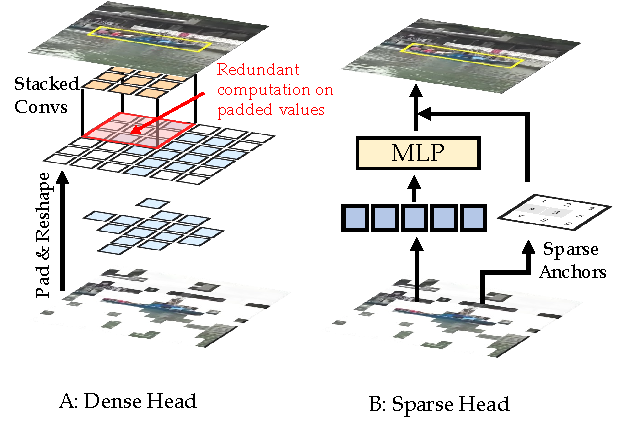
\includegraphics[width=0.5\textwidth, trim=4pt 5pt 0pt 0pt, clip]{imgs/sparse_head.pdf}
    \caption{\textbf{Dense vs.\ sparse prediction head.}
    (A)~Dense head pads and reshapes sparse tokens into a full 2D grid, wasting computation on empty positions.
    (B)~Our sparse head applies an MLP directly on retained tokens via sparse anchors, with no padding or reshape.}
    \label{fig:sparse_head}
    \vspace{-0.5em}
\end{wrapfigure}
Our goal is to avoid the dense-head bottleneck when the backbone operates on a sparsified, unstructured token set. Let the retained search tokens be
\(\mathcal{L}_K = \{\mathbf{f}_k\}_{k=1}^{N_K}\), where $N_K\ll H_xW_x/P^2$ and each token keeps its original 2D location on the patch grid, denoted as $\mathbf{p}_k=(u_k,v_k)$.
As illustrated in~\figref{fig:sparse_head}, unlike dense heads that must pad and reshape sparse tokens back to a full 2D grid before stacked convolutions, we design a natively sparse head that directly consumes $\mathcal{L}_K$ without padding or reshaping back to a dense feature map.
We parameterize both branches with lightweight MLPs, similar to prior MLP-based heads (e.g., LoRAT~\cite{lin2024loratrack}). We further tailor the head for sparse token decoding via a score-first, regress-once computation path.

\textbf{Score-first, regress-once.} As illustrated in~\figref{main_frame}, the head contains two lightweight branches.
\begin{itemize}
  \item \textbf{Score branch} $g_{\text{s}}$ predicts a scalar confidence $s_k\in\mathbb{R}$ for each retained token.
      The target token is selected by
      \begin{equation}
        k^* = \arg\max_k\; s_k.
      \end{equation}
      This selection can be implemented by scattering $\{s_k\}$ to a sparse score map aligned with the original grid and applying an \texttt{ArgMax}, but no dense feature computation is required.

  \item \textbf{Regression branch} $g_{\text{r}}$ predicts box parameters only \emph{once} for the selected token $\mathbf{f}_{k^*}$.
      Denoting the regression output as $\Delta_{k^*}$, the final box is decoded as
      \begin{equation}
        \hat{\mathbf{b}} = \mathrm{Decode}(\mathbf{p}_{k^*},\, \Delta_{k^*}).
      \end{equation}
\end{itemize}

Importantly, the anchor point $\mathbf{p}_{k^*}$ is directly retrieved from the retained token's stored coordinate (i.e., a sparse map lookup), avoiding any padding/reshape to dense 2D feature maps; meanwhile, no regression is computed for other tokens.

This design makes the head complexity scale with $N_K$ for scoring and constant-time for regression, matching the sparsified backbone and eliminating redundant computation on empty spatial positions.

\textbf{Training objective.} We supervise the score branch with a classification loss over sparse tokens, and supervise the regression branch on a single token aligned with the ground-truth target.
Let $\mathbf{c}$ be the ground-truth target center on the patch grid and define
\begin{equation}
  k^{\text{gt}} = \arg\min_k \lVert \mathbf{p}_k - \mathbf{c} \rVert_2.
\end{equation}
The overall head loss is
\begin{equation}
  L_{\text{head}} = L_{\text{cls}}(\{s_k\}) + \lambda_{\ell_1} L_{\ell_1}(\hat{\mathbf{b}}_{k^{\text{gt}}}, \mathbf{b}) + \lambda_{\text{GIoU}} L_{\text{GIoU}}(\hat{\mathbf{b}}_{k^{\text{gt}}}, \mathbf{b}),
\end{equation}
where $\mathbf{b}$ is the ground-truth box, and we set $\lambda_{\text{GIoU}} = 2$ and $\lambda_{\ell_1}=5$.
